% Double-anonymous ICSEC 2026 review manuscript.
\documentclass[conference]{IEEEtran}
\usepackage[T1]{fontenc}
\usepackage{graphicx}
\usepackage{booktabs}
\usepackage{multirow}
\usepackage{amsmath}
\usepackage{cite}
\usepackage{xcolor}
\usepackage{tikz}
\usetikzlibrary{arrows.meta,positioning,shapes.geometric,fit}
\usepackage[hidelinks,pdftitle={Genetic Optimization of Three-Way Operational Decisions for Cross-Platform Profile Identity Resolution},pdfauthor={Anonymous},pdfsubject={Double-anonymous ICSEC 2026 submission},pdfkeywords={entity resolution, record linkage, evolutionary computing}]{hyperref}
\newcommand{\pmv}{\,$\pm$\,}
\begin{document}
\title{Genetic Optimization of Three-Way Operational Decisions for Cross-Platform Profile Identity Resolution}
\author{\IEEEauthorblockN{Anonymous Submission}}
\maketitle

\begin{abstract}
Cross-platform identity resolution must link incomplete social-media profiles while controlling false merges, missed matches, and cases retained for review. Pair classifiers supply scores, but deployment requires a policy that separates automatic matches, rejections, and uncertain cases. This paper evaluates a staged profile-linkage pipeline on a transformed derivative of the LinkSocial corpus containing Twitter, Google+, and Instagram profiles. A Gradient Boosting baseline using 17 handcrafted profile-pair features (GB-17) is compared with an augmentation by MiniLM cosine similarity (GB-18). A genetic algorithm selects a four-parameter MATCH/REVIEW/NO\_MATCH policy on validation entities while retaining calibrated GB-18 probabilities unchanged. Evaluation uses three repeated outer entity-disjoint partitions with distinct model-training, calibration, policy-selection, and test entities. The GA policy achieves mean F1 of 0.8603 versus 0.8280 for fixed-threshold GB-18, and lowers a declared illustrative utility from 2271.8 to 1802.7. It also increases mean false positives from 38.0 to 75.7 and review decisions from 438.0 to 923.3. The MiniLM fixed-threshold ablation is mixed across outer splits. Candidate generation covers 88.6742\% of 29,243 labeled positive pairs, limiting attainable end-to-end recall. Findings are limited to LinkSocial and the declared utility scenario.
\end{abstract}

\begin{IEEEkeywords}
entity resolution, record linkage, cross-platform identity linkage, evolutionary computing, operational decision policy, machine learning
\end{IEEEkeywords}

\section{Introduction}
People may maintain profiles on multiple social platforms while identifiers, names, biographies, links, and locations differ or are incomplete. Linking these profiles supports data integration but creates asymmetric risks: incorrect merges and missed links have different operational consequences. Profile linkage commonly uses similarity features and supervised pair classification \cite{sharma2018linksocial,yao2023profile}. Candidate generation is also necessary because exhaustive entity-resolution (ER) comparison is quadratic \cite{papadakis2021blocking,li2020blocking}.

A pair score does not itself specify an operating decision. A system must decide whether to accept a pair, reject it, or retain it for review. Three-way record linkage is established \cite{ouyang2019threeway}, as are evolutionary approaches to ER \cite{sun2017gaer}. Thus, this work does not claim novelty for genetic algorithms (GAs) or three-way linkage. Instead, it evaluates a separated operational composition: semantic-enhanced calibrated pair scoring followed by validation-only genetic selection of a three-way policy under entity-disjoint evaluation.

We ask: \textit{RQ1}, how does a MiniLM cosine feature affect fixed-threshold workflow outcomes? \textit{RQ2}, given frozen calibrated GB-18 probabilities, how does a GA-selected three-way policy alter precision, recall, F1, review volume, and an illustrative utility? \textit{RQ3}, how strongly does candidate-generation recall constrain end-to-end resolution? Contributions are: 1) an entity-disjoint protocol separating training, calibration, policy selection, and testing; 2) controlled representation and decision-policy ablations; 3) repeated outer-split evidence for the policy trade-off; and 4) retrieval-to-decision failure decomposition.

\section{Related Work}
Blocking and filtering reduce ER candidate sets but may exclude true pairs, making candidate coverage distinct from downstream classification \cite{papadakis2021blocking,li2020blocking}. This motivates reporting retrieval recall and blocking misses separately from scoring results. Profile-based user identity linkage uses string, short-text, and semi-structured attributes with machine-learning models \cite{yao2023profile}.

Three-way record linkage has been studied through granular descriptors \cite{ouyang2019threeway}, while GA-based ER with active learning has also been studied \cite{sun2017gaer}. These works preclude claims that the basic decision formulation or evolutionary method is new. Application-specific linkage evaluation can require more than a single aggregate classification measure \cite{christen2026consistent}; accordingly, this study reports FP, FN, review count, precision, recall, F1, and declared utility together. Its contribution is empirical evidence for a staged composition, not a claim of the first combination of calibrated probabilities, semantic features, and a GA policy.

\section{Methodology}
\subsection{Data, Labels, and Candidate Generation}
Experiments use a locally transformed derivative of the public LinkSocial corpus \cite{sharma2018linksocial}, with 36,807 profiles from Twitter, Google+, and Instagram. A positive pair has the same non-empty source entity identifier. The public source documents usernames, full names, biographies, external URLs, bi-grams, and profile-image URLs for some platforms \cite{sharma2018linksocial}. The source repository does not state a machine-readable reuse license or formal ethics documentation; raw records are not redistributed.

Candidate generation combines an exact tier with username-prefix, full-name-prefix, and external-domain blocking. It retains 2,086,245 pairs from 449,149,239 possible cross-platform comparisons. Of 29,243 labeled positive pairs, 25,931 enter the candidate workflow and 3,312 do not, yielding retrieval recall 0.886742.

\subsection{Pair Models and Decision Policy}
GB-17 uses a Gradient Boosting classifier with 17 handcrafted pair features: username/full-name Jaro, normalized Levenshtein, and token similarities; cross-field name similarity; bio overlap/length features; location features; platform and availability indicators; and length/prefix features. GB-18 adds only $\mathrm{bert\_cos}$, cosine similarity of normalized \texttt{all-MiniLM-L6-v2} embeddings of concatenated full name, biography, and location.

Both variants use 300 estimators, learning rate 0.05, maximum depth 6, and seed 42. Training negatives are deterministically undersampled to a 3:1 negative-to-positive ratio. Isotonic regression is fitted only on calibration entities. The fixed policy assigns MATCH for probability at least 0.98, REVIEW for $[0.95,0.98)$, and NO\_MATCH otherwise.

GB-18-GA retains persisted calibrated GB-18 probabilities unchanged; it neither updates the classifier nor refits the calibrator. For calibrated probability $p$ and name evidence $n$, the genome $g=[t_m,t_r,c_p,c_d]$ applies MATCH for $p\geq t_m$; within $t_r\leq p<t_m$, it applies MATCH for $n\geq c_p$, NO\_MATCH for $n<c_d$, and REVIEW otherwise; it applies NO\_MATCH for $p<t_r$. Constraints are $0.90\leq t_m\leq0.999$, $0.50\leq t_r\leq t_m$, $0.50\leq c_p\leq1$, and $0\leq c_d\leq c_p$.

The GA uses five seeds $\{7,42,123,999,2025\}$, population 60, 40 generations, 12 elites, uniform crossover, and Gaussian mutation with probability 0.30 and standard deviation 0.02. Validation-only selection minimizes the illustrative objective
\begin{equation}
U=2\,FP+FN+0.1\,REVIEW.
\end{equation}
This is a declared operational scenario, not a measured economic cost. All component metrics are reported alongside $U$.

\section{Experimental Setup}
For each deterministic outer partition (seeds 101, 202, and 303), an MD5-based rule assigns approximately 30\% of entities to outer test. Remaining entities are allocated to model training (70\%), calibration (15\%), and GA validation (15\%). Cross-role candidate pairs are dropped, and the implementation asserts no entity overlap. Test labels are not accessed during training, calibration, GA optimization, or seed selection.

The role counts before scored-pair filtering in the frozen primary run were 510,981 training, 26,246 calibration, 22,873 GA-validation, and 195,440 test candidate pairs; 1,330,705 cross-role candidates were dropped. Figure~\ref{fig:pipeline} summarizes the protocol. Workflow-level metrics include split-specific exact-tier outputs and blocking-missed positives as fixed constants. We report mean and standard deviation across outer partitions. On a separately frozen primary test role, a 2,000-resample paired conditional bootstrap estimates uncertainty over scored candidates while retaining exact/blocking constants fixed.

\begin{figure*}[!t]
\centering
\resizebox{\textwidth}{!}{%
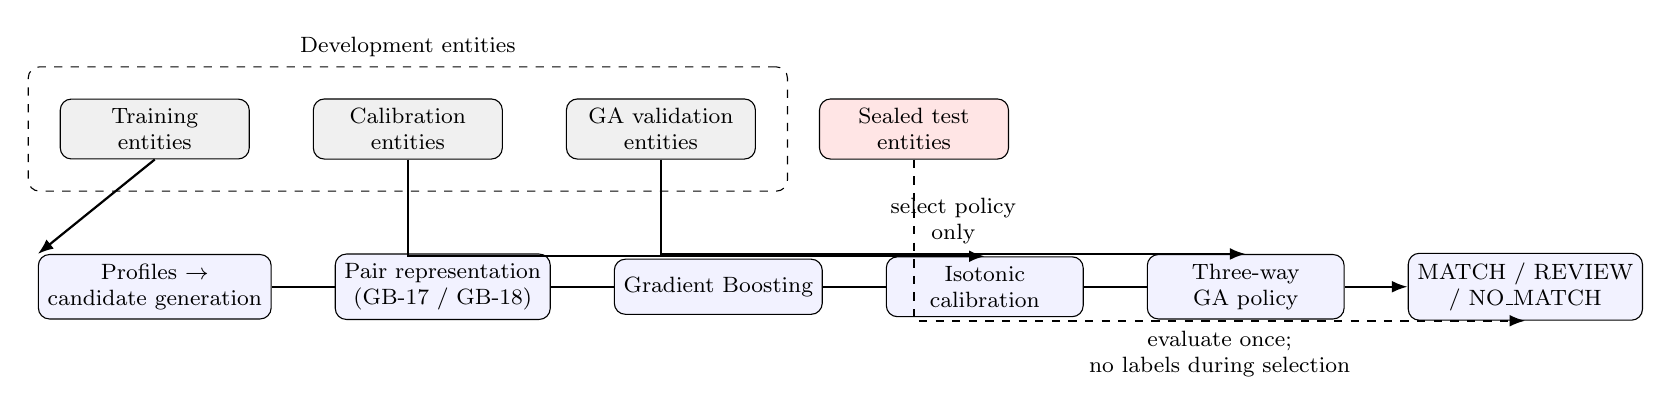
\begin{tikzpicture}[font=\footnotesize, node distance=4mm and 8mm,
block/.style={draw, rounded corners, align=center, minimum width=25mm, minimum height=7mm, fill=blue!5},
role/.style={draw, rounded corners, align=center, minimum width=24mm, minimum height=7mm, fill=gray!12},
arrow/.style={-{Latex[length=2mm]}, thick}]
\node[role] (train) {Training\\entities};
\node[role,right=of train] (cal) {Calibration\\entities};
\node[role,right=of cal] (val) {GA validation\\entities};
\node[role,right=of val,fill=red!10] (test) {Sealed test\\entities};
\node[block,below=12mm of train] (cand) {Profiles $\rightarrow$\\candidate generation};
\node[block,right=of cand] (repr) {Pair representation\\(GB-17 / GB-18)};
\node[block,right=of repr] (gb) {Gradient Boosting};
\node[block,right=of gb] (iso) {Isotonic\\calibration};
\node[block,right=of iso] (ga) {Three-way\\GA policy};
\node[block,right=of ga] (out) {MATCH / REVIEW\\/ NO\_MATCH};
\draw[arrow] (train.south) -- (cand.north west);
\draw[arrow] (cand) -- (repr) -- (gb) -- (iso) -- (ga) -- (out);
\draw[arrow] (cal.south) |- (iso.north);
\draw[arrow] (val.south) |- node[pos=.75,above,align=center]{select policy\\only} (ga.north);
\draw[arrow,dashed] (test.south) |- node[pos=.75,below,align=center]{evaluate once;\\no labels during selection} (out.south);
\node[draw,dashed,rounded corners,fit=(train)(cal)(val),inner sep=4mm,label=above:{Development entities}] {};
\end{tikzpicture}%
}
\caption{Leakage-safe evaluation pipeline. The GA uses validation entities only; sealed-test labels are accessed only for final evaluation.}
\label{fig:pipeline}
\end{figure*}

\section{Results and Discussion}
\subsection{Repeated Outer-Split Evaluation}
\begin{table*}[!t]
\caption{Repeated outer-split workflow performance (mean $\pm$ SD over three partitions). $U$ is the illustrative utility in (1).}
\label{tab:performance}
\centering\small
\begin{tabular}{lccccccc}
\toprule
Method & Precision & Recall & F1 & FP & FN & Review & $U$\\
\midrule
GB-17 & .9909\pmv.0051 & .7137\pmv.0431 & .8292\pmv.0277 & 59.0\pmv35.8 & 2266.3\pmv113.4 & 264.7\pmv395.9 & 2410.8\pmv98.9\\
GB-18 & .9940\pmv.0010 & .7099\pmv.0322 & .8280\pmv.0222 & 38.0\pmv7.0 & 2152.0\pmv232.6 & 438.0\pmv406.1 & 2271.8\pmv198.5\\
GB-18-GA & .9889\pmv.0054 & .7614\pmv.0028 & .8603\pmv.0011 & 75.7\pmv38.4 & 1559.0\pmv38.1 & 923.3\pmv151.1 & 1802.7\pmv68.3\\
\bottomrule
\end{tabular}
\end{table*}

\begin{table*}[!t]
\caption{Per-outer-partition F1 and illustrative utility. Each outer test partition is entity-disjoint from its corresponding training, calibration, and GA-validation entities.}
\label{tab:perouter}
\centering\small
\begin{tabular}{crrrrrr}
\toprule
Outer seed & \multicolumn{2}{c}{GB-17} & \multicolumn{2}{c}{GB-18} & \multicolumn{2}{c}{GB-18-GA}\\
& F1 & $U$ & F1 & $U$ & F1 & $U$\\
\midrule
101 & .8394 & 2523.2 & .8408 & 2051.2 & .8616 & 1759.2\\
202 & .7978 & 2337.0 & .8408 & 2436.0 & .8600 & 1767.4\\
303 & .8504 & 2372.2 & .8023 & 2328.2 & .8594 & 1881.4\\
\bottomrule
\end{tabular}
\end{table*}

RQ1 produces mixed evidence. On the separately frozen primary split, GB-18 raises F1 from 0.5963 to 0.8387. Across repeated outer splits, however, fixed-threshold GB-18 does not consistently exceed GB-17: F1 by seed is .8408/.8408/.8023 for GB-18 versus .8394/.7978/.8504 for GB-17. MiniLM cosine is therefore a controlled representation component, not a consistently superior fixed-threshold method on this corpus.

For RQ2, GB-18-GA exceeds GB-18 F1 in each outer partition, by 0.0208, 0.0192, and 0.0571. Mean recall rises from .7099 to .7614 and mean FN decreases from 2152.0 to 1559.0. This occurs with higher FP and review volume. The GA policy changes the operating trade-off; it is not uniformly better in every error dimension.

\begin{table}[!t]
\caption{GB-18-GA scored-candidate test slices in the frozen primary run. These rows exclude split-level exact/blocking constants.}
\label{tab:platform}
\centering\footnotesize
\begin{tabular}{lrrrr}
\toprule
Platform pair & Precision & Recall & F1 & FP/FN\\
\midrule
Google+--Instagram & .9831 & .7647 & .8603 & 21/192\\
Google+--Twitter & .9806 & .7204 & .8306 & 28/291\\
Instagram--Twitter & .8837 & .7580 & .8160 & 47/76\\
\bottomrule
\end{tabular}
\end{table}

The Instagram--Twitter slice has lower scored-candidate precision than the other platform-pair slices. This heterogeneous error profile motivates reporting platform-pair detail rather than inferring uniform behavior from an aggregate score.

On the primary frozen split, conditional paired-bootstrap intervals for GB-18-GA minus GB-18 exclude zero for F1 (+.0235, 95\% CI [.0208,.0262]), recall (+.0386, [.0344,.0427]), FP (+32, [+22,+44]), FN (-266, [-299,-234]), REVIEW (+224, [+166,+283]), and $U$ (-179.6, [-214.7,-144.1]). These intervals condition on one scored test population and fixed retrieval constants; they are not population-level significance claims.

\subsection{Candidate-Generation Ceiling}
\begin{table}[!t]
\caption{Candidate-generation and retrieval decomposition.}
\label{tab:retrieval}
\centering\small
\begin{tabular}{lr}
\toprule
Measure & Value\\
\midrule
Possible cross-platform pairs & 449,149,239\\
Candidate pairs & 2,086,245\\
Space reduction & 99.5355\%\\
Labeled positive pairs & 29,243\\
Covered positives & 25,931\\
Blocking misses & 3,312\\
Retrieval recall & 88.6742\%\\
\bottomrule
\end{tabular}
\end{table}

RQ3 establishes a pipeline limitation, not a retrieval improvement. The 3,312 positives absent from candidates cannot be corrected by GB-17, GB-18, or GB-18-GA. Across outer tests, candidate recall is .8838\pmv.0002 with 1023.7\pmv10.2 blocking-missed positives. Pair-model improvements must not be interpreted as complete end-to-end resolution improvements.

A 12-scenario frozen-policy sensitivity analysis varies FP penalty $\{1,2,5,10\}$ and REVIEW penalty $\{.02,.1,.5\}$, fixing FN penalty at 1. GB-18-GA has lowest utility in 8 of 12 scenarios, not all. Policies were not retuned after changing scenarios; this is sensitivity analysis, not a new policy-selection result.

\subsection{Failure Modes}
The frozen primary test analysis distinguishes workflow errors from scored-candidate errors. Of 96 scored-candidate false-positive MATCH decisions under GB-18-GA, 66 occur in the high name-similarity band; the remaining workflow FP count also includes fixed exact-tier errors. Thus, lexical agreement remains a false-merge risk rather than sufficient identity proof.

Among 559 scored-candidate false-negative NO\_MATCH decisions, 242 lack paired biography evidence and 236 lack usable paired URL evidence. All 559 lack paired usable location evidence in the reconstructed test representation. These counts do not imply that missing fields cause every error, but they show that several secondary evidence channels are unavailable where decisions fail.

The review region contains 480 positive and 367 negative scored candidates. It therefore contains both recoverable matches and likely nonmatches, rather than a homogeneous deferred class. This supports retaining REVIEW as an explicit operational outcome, while also showing that its practical usefulness requires a separate human-review study.

\section{Limitations and Threats to Validity}
The study evaluates one transformed corpus and does not establish outcomes for other platforms, languages, time periods, or datasets. Only three outer partitions are used. Source labels may contain noise. Utility coefficients are illustrative assumptions, not measured business cost. Candidate blocking omits positives before scoring, and no improved blocking method is proposed. REVIEW is an offline policy output, not observed human-review workload or accuracy.

The public LinkSocial repository identifies the source corpus but lacks a machine-readable license and formal ethics documentation in inspected materials. This study does not claim redistribution rights, consent, or ethical approval. Reproducibility materials should be restricted to code where permitted, configurations, hashes, aggregate results, and non-identifying error categories; raw profiles and decision data must not be released without source-owner permission.

Internal validity is strengthened by assigning entities, rather than pairs, to roles and dropping cross-role pairs. Nevertheless, labels derived from a shared source entity identifier can contain errors that are not independently adjudicated. Construct validity is limited because the offline REVIEW label measures a policy outcome, not analyst accuracy, review time, or reviewer agreement. The conditional bootstrap estimates uncertainty over scored candidates in one frozen test population while holding exact-tier and blocking-miss constants fixed; it should not be interpreted as an independent resampling of the entire corpus.

External validity is limited by the three historical social platforms and their archived profile fields. Platform-pair differences in Table~\ref{tab:platform} show that aggregate performance can conceal heterogeneous error behavior. Conclusion validity is also sensitive to the declared utility coefficients: the 12-scenario analysis shows that GB-18-GA is not preferred for every FP/FN/REVIEW penalty combination. These boundaries motivate reporting the component outcomes rather than treating the utility as a general business measure.

\section{Conclusion}
This work evaluated a staged cross-platform profile-linkage pipeline in which a GA selects a three-way operating policy over frozen calibrated pair probabilities. Across three repeated entity-disjoint outer splits, the policy improved F1, recall, and the declared utility scenario relative to fixed-threshold GB-18, while increasing false positives and review outcomes. The MiniLM fixed-threshold ablation showed mixed repeated-split behavior. Candidate coverage remained binding: approximately 11.3\% of labeled positive pairs were unavailable to downstream scoring. These findings support a bounded operating trade-off on LinkSocial, not a new GA or three-way linkage method, universal utility reduction, or generalization beyond the evaluated corpus.

\bibliographystyle{IEEEtran}
\bibliography{references}
\end{document}
